\documentclass[./../main.tex]{subfiles}
\graphicspath{{img/}}

\begin{document}
    \begin{exercise}[Cadena monoatómica con acoplamiento entre segundos vecinos]
        Considera una cadena unidimensional de átomos idénticos de masa \(m\). Cada átomo está unido con su vecino a través de un resorte de constante \(\kappa_{1}\). Considera además que cada átomo también está conectado con su segundo vecino por medio de un segundo resorte de constante \(\kappa_{2}\), como se ilustra en la \cref{fig:monoatomicChain}.

        \begin{figure}[htb]
            \centering
            % \includegraphics[height=0.3\textwidth, width=0.8\textwidth]{example-image-a}
            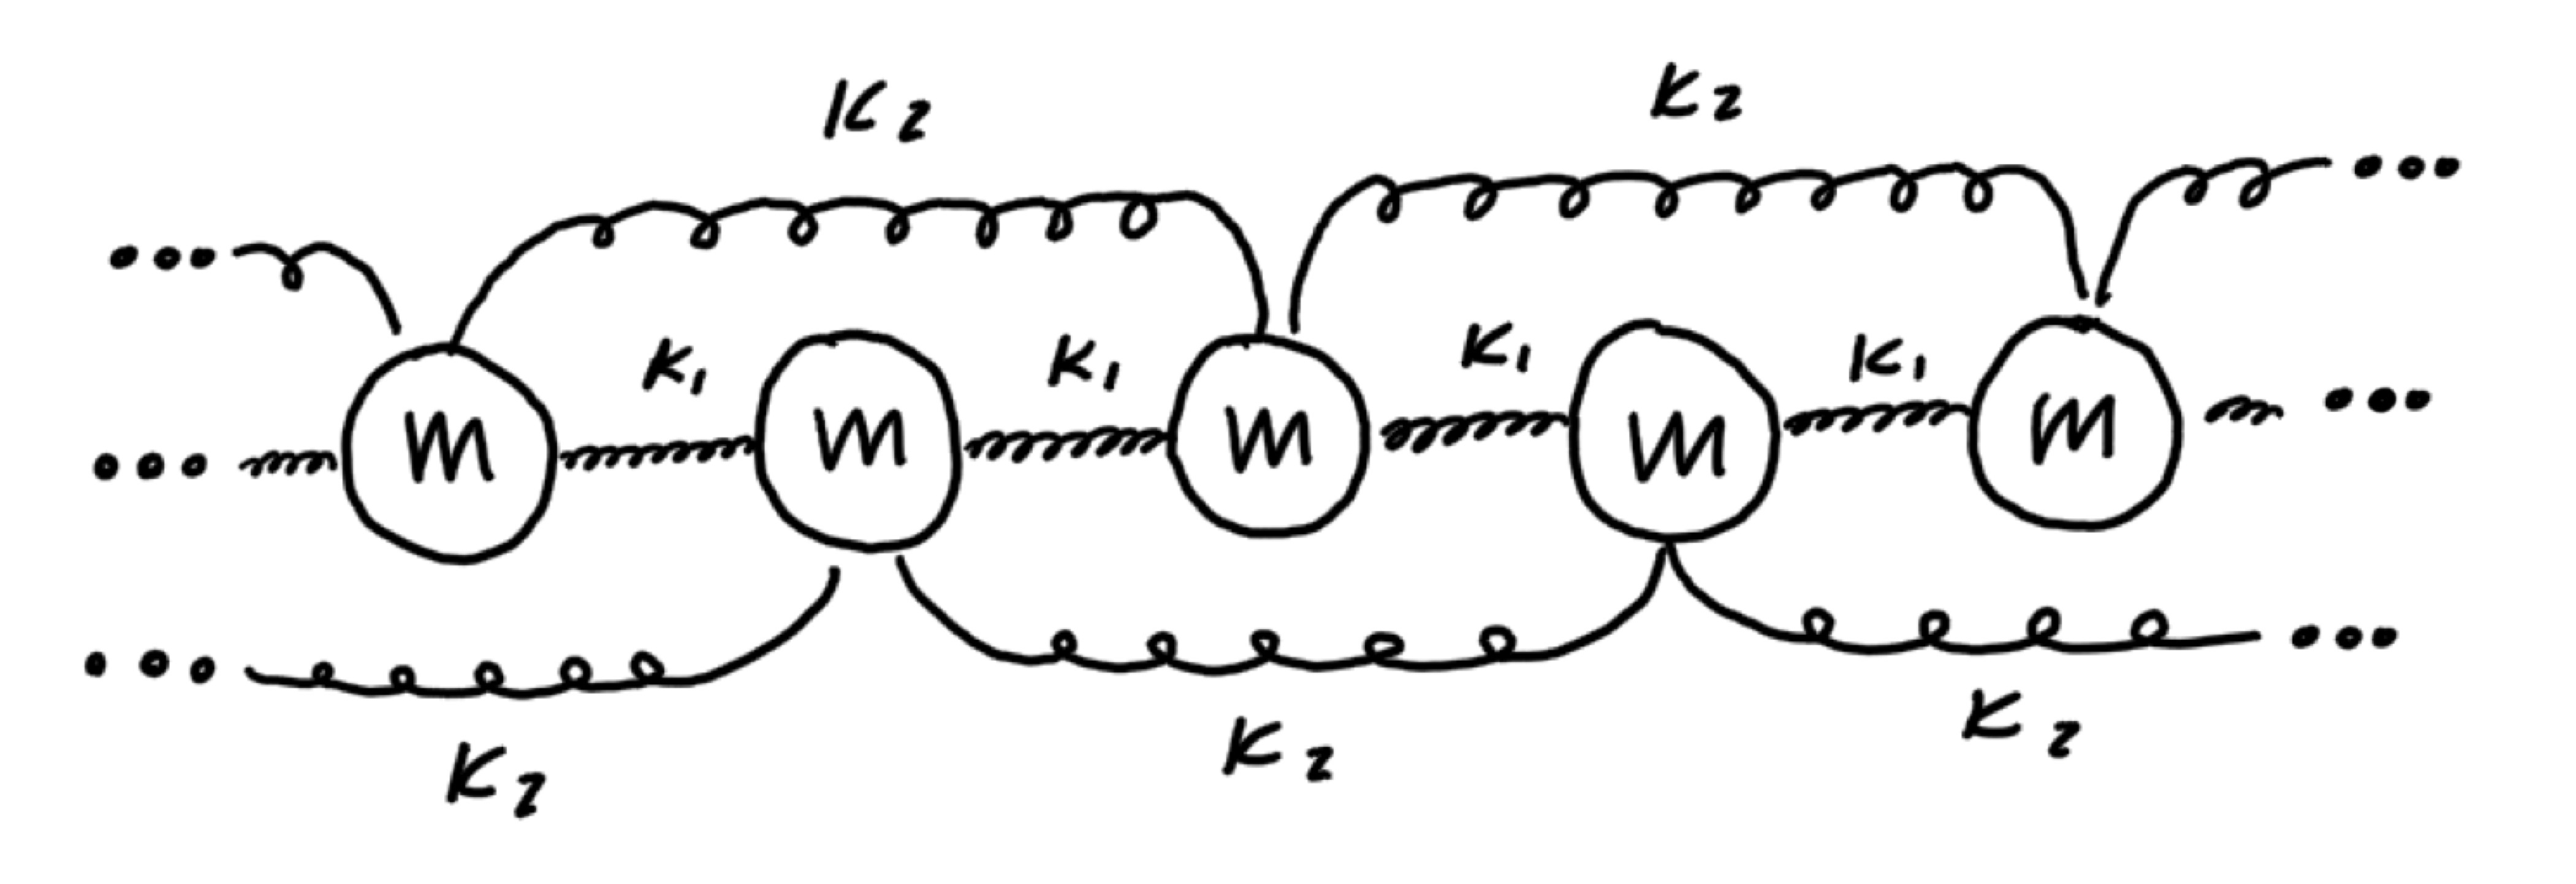
\includegraphics[width=0.6\textwidth]{monatomic-chain}
            \caption{Cadena monoatómica con acoplamiento entre primeros y segundos vecinos.}
            \label{fig:monoatomicChain}
        \end{figure}

        \begin{enumerate}
            \item (Valor: 2.5pt) - Muestra que la ecuación de movimiento asociada al desplazamiento \(\fdif{x_{n}}\), de la \(n\)-ésima masa es:
            
            \begin{equation*}
                m\fdif{\ddot{x}_{n}} = \kappa_{1}(\fdif{x_{n + 1}} - \fdif{x_{n}}) + \kappa_{1}(\fdif{x_{n - 1}} - \fdif{x_{n}}) + \kappa_{2}(\fdif{x_{n + 2}} - \fdif{x_{n}}) + \kappa_{2}(\fdif{x_{n - 2}} - \fdif{x_{n}})
            \end{equation*}

            \begin{solution}
                Sabemos que la energía potencial de la cadena está dada por:

                \begin{equation*}
                    V_{\text{tot}} = \sum_{i}\dfrac{\kappa}{2}(\fdif{x_{i + 1}} - \fdif{x_{i}})^{2},
                \end{equation*}

                esto para cada una de las constantes de los resortes.

                Así,

                \begin{equation*}
                    V_{\text{tot}} = \dfrac{\kappa_{1}}{2}\left[(\fdif{x_{n + 1}} -\fdif{x_{n}})^{2} + (\fdif{x_{n}} - \fdif{x_{n - 1}})^{2}\right]
                    + \dfrac{\kappa_{2}}{2}\left[(\fdif{x_{n + 2}} - \fdif{x_{n}})^{2} + (\fdif{x_{n}} - \fdif{x_{n - 2}})^{2}\right]
                \end{equation*}

                \pagebreak
                La fuerza sobre la \(n\)-ésima masa está dada como

                \begin{align*}
                    F_{n} = -\pdv{V_{\text{tot}}}{x_{n}} &= 
                    \begin{multlined}[t]
                        -\dfrac{\kappa_{1}}{2}\left[2(\fdif{x_{n + 1}} - \fdif{x_{n}})\cdot (-1)
                    + 2(\fdif{x_{n}} - \fdif{x_{n - 1}})\right]\\
                    - \dfrac{\kappa_{2}}{2}\left[2(\fdif{x_{n + 2}} - \fdif{x_{n}})\cdot(-1) + 2(\fdif{x_{n}} - \fdif{x_{n - 2}})\right],
                    \end{multlined}\\
                    F_{n} &= \kappa_{1}(\fdif{x_{n + 1}} - \fdif{x_{n}}) + \kappa_{1}(\fdif{x_{n - 1}} - \fdif{x_{n}}) + \kappa_{2}(\fdif{x_{n + 1}} - \fdif{x_{n}}) + \kappa_{2}(\fdif{x_{n - 2}} - \fdif{x_{n}}).
                \end{align*}

                Y \(F = ma = m\odv[order=2]{x}{t}\), entonces

                \begin{empheq}[box=\resultbox]{equation}
                    m\fdif{\ddot{x}_{n}} = \kappa_{1}(\fdif{x_{n + 1}} - \fdif{x_{n}}) + \kappa_{1}(\fdif{x_{n - 1}} - \fdif{x_{n}}) + \kappa_{2}(\fdif{x_{n + 2}} - \fdif{x_{n}}) + \kappa_{2}(\fdif{x_{n - 2}} - \fdif{x_{n}}).
                    \label{eq:EOMMonatomicChain}
                \end{empheq}
            \end{solution}

            \item (Valor: 2.5pt) - Usando el resultado del inciso anterior, demuestra que la relación de dispersión \(\omega(k)\) para este modelo está dada por:
            
            \begin{equation*}
                \omega(k) = \sqrt{\dfrac{2\kappa_{1}}{m}(1 - \cos(ka)) + \dfrac{2\kappa_{2}}{m}(1 - \cos(2ka))}
            \end{equation*}

            en donde \(a\) es la constante de la red (es decir, la separación entre átomos).

            \begin{solution}
                Buscamos soluciones para los modos normales. Tenemos el ansatz,

                \begin{equation*}
                    \fdif{x_{n}} = A\e^{\i\omega t - \i kna}.
                \end{equation*}

                Sustituimos en \cref{eq:EOMMonatomicChain},

                \begin{align*}
                    -m\omega^{2}A\e^{-\i\omega t - \i kna} &=
                    \begin{multlined}[t]
                        \kappa_{1}\left(A\e^{-\i\omega t - \i k(n + 1)a} - A\e^{-\i\omega t - \i kna}
                        \right)
                        + \kappa_{1}\left(A\e^{-\i\omega t -\i k(n - 1)a} - A\e^{-\i\omega t - \i kna}\right)\\
                        + \kappa_{2}\left(A\e^{-\i\omega t -\i k(n + 2)a} - A\e^{-\i\omega t - \i kna}\right)
                        + \kappa_{2}\left(A\e^{-\i\omega t - \i k(n - 2)a} - A\e^{-\i\omega t -\i kna}\right),
                    \end{multlined}\\
                    &= 
                    \begin{multlined}[t]
                        A\kappa_{1}\e^{-\i\omega t}\left[\e^{-\i kna}\e^{-\i ka} - \e^{-\i kna} + \e^{-\i kna}\e^{+\i ka} - \e^{-\i kna}\right],\\
                        + A\kappa_{2}\e^{-\i\omega t}\left[\e^{-\i kna}\e^{-\i2ka} - \e^{-\i kna} + \e^{-\i kna}\e^{+\i2ka} - \e^{-\i kna}\right],
                    \end{multlined}\\
                    &= A\e^{-\i\omega t - \i kna}\left[\kappa_{1}(\e^{-\i ka} + \e^{\i ka} - 2) + \kappa_{2}(\e^{-\i2ka} + \e^{\i2ka} - 2)\right].
                \end{align*}

                Usamos que \(\cos(x) = \tfrac{1}{2}(\e^{\i x} + \e^{-\i x})\),

                \begin{align*}
                    \implies &= A\e^{-\i\omega t - \i kna}\left[k_{1}(2\cos(x) - 2) + \kappa_{2}(2\cos(2ka) - 2)\right] = -m\omega^{2}A\e^{-\i\omega t - \i kna},\\
                    m\omega^{2} &= 2\kappa_{1}(1 - \cos(ka)) + 2\kappa_{2}(1 - \cos(2ka)).
                \end{align*}

                Por lo que la relación de dispersión es

                \begin{empheq}[box=\resultbox]{equation}
                    \omega(k) = \sqrt{\tfrac{2\kappa_{1}}{m}(1 - \cos(ka)) + \tfrac{2\kappa_{2}}{m}(1 - \cos(2ka))}.
                    \label{eq:DispersionRelation}
                \end{empheq}
            \end{solution}
            
            \item (Valor: 2.5pt) - Grafica esta relación de dispersión dentro de la primera zona de Brillouin.
            
            Al intervalo \(-\tfrac{\pi}{a} \leq k \leq \tfrac{\pi}{a}\) se conoce como la primera zona de Brillouin. Para graficar la relación de dispersión \cref{eq:DispersionRelation} se usaron los siguientes parámetros: \(\kappa_{1} = 100\), \(\kappa_{2} = 1\), \(m = 1\), \(a = 1\). La gráfica se muestra en la \cref{fig:DispersionRelationPlot}.

            \begin{figure}[htb]
                \centering
                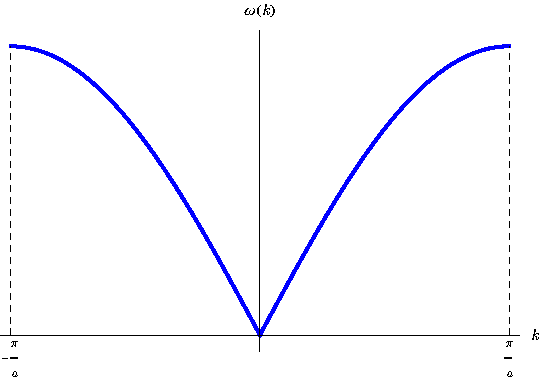
\includegraphics[width=.8\textwidth]{FirstBrillouinZone.pdf}
                \caption{Relación de dispersión \(\omega(k)\) en la primera zona de Brillouin.}
                \label{fig:DispersionRelationPlot}
            \end{figure}
            
            \item (Valor: 2.5pt) - Usando el resultado del inciso (b), demuestra que la velocidad del sonido está dada por:
            
            \begin{equation*}
                v_{s} = a\sqrt{\dfrac{\kappa_{1} + 4\kappa_{2}}{m}}
            \end{equation*}

            \begin{solution}
                Para las ondas sonoras \(\omega_{s}(k) \propto k\),

                \begin{equation*}
                    \omega_{s}(k) = v_{s}k,
                \end{equation*}

                para \(k\) pequeña.

                Recordamos además que
                
                \begin{equation*}
                    2\sin^{2}\left(\tfrac{x}{2}\right) = 1 - \cos(x).
                \end{equation*}

                Así, \cref{eq:DispersionRelation} queda como:

                \begin{equation*}
                    \omega(k) = \sqrt{\tfrac{4\kappa_{1}}{m}\sin^{2}\left(\tfrac{ka}{2}\right) + \tfrac{4\kappa_{2}}{m}\sin^{2}\left(ka\right)}.
                \end{equation*}

                Usando que \(\sin(x) \simeq x\) para \(x\) pequeña.

                \begin{align*}
                    \omega(k) &\simeq \sqrt{\tfrac{4\kappa_{1}}{m}\left(\tfrac{ka}{2}\right)^{2} + \tfrac{4\kappa_{2}}{m}(ka)^{2}},\\
                    &= \sqrt{(ka)^{2}\left(\dfrac{k_{1} + 4\kappa_{2}}{m}\right)},\\
                    \implies \omega(k) &= a\sqrt{\dfrac{\kappa_{1} + 4\kappa_{2}}{m}}k.
                \end{align*}

                Por lo que la velocidad del sonido es

                \begin{empheq}[box=\resultbox]{equation*}
                    v_{s} = a\sqrt{\dfrac{\kappa_{1} + 4\kappa_{2}}{m}}.
                \end{empheq}
            \end{solution}
        \end{enumerate}
    \end{exercise}
\end{document}